%% Version 4.3.1, 19 May 2014
%
%%%%%%%%%%%%%%%%%%%%%%%%%%%%%%%%%%%%%%%%%%%%%%%%%%%%%%%%%%%%%%%%%%%%%%
% Template.tex --  LaTeX-based template for submissions to the 
% American Meteorological Society
%
% Template developed by Amy Hendrickson, 2013, TeXnology Inc., 
% amyh@texnology.com, http://www.texnology.com
% following earlier work by Brian Papa, American Meteorological Society
%
% Email questions to latex@ametsoc.org.
%
%%%%%%%%%%%%%%%%%%%%%%%%%%%%%%%%%%%%%%%%%%%%%%%%%%%%%%%%%%%%%%%%%%%%%
% PREAMBLE
%%%%%%%%%%%%%%%%%%%%%%%%%%%%%%%%%%%%%%%%%%%%%%%%%%%%%%%%%%%%%%%%%%%%%

%% Start with one of the following:
% DOUBLE-SPACED VERSION FOR SUBMISSION TO THE AMS
%\documentclass{ametsoc}

% TWO-COLUMN JOURNAL PAGE LAYOUT---FOR AUTHOR USE ONLY
 \documentclass[draft]{ametsoc}
 \usepackage[colorinlistoftodos]{todonotes}
%%%%%%%%%%%%%%%%%%%%%%%%%%%%%%%%
%%% To be entered only if twocol option is used

\journal{bams}

%  Please choose a journal abbreviation to use above from the following list:
% 
%   jamc     (Journal of Applied Meteorology and Climatology)
%   jtech     (Journal of Atmospheric and Oceanic Technology)
%   jhm      (Journal of Hydrometeorology)
%   jpo     (Journal of Physical Oceanography)
%   jcli      (Journal of Climate)
%   mwr      (Monthly Weather Review)
%   wcas      (Weather, Climate, and Society)
%   waf       (Weather and Forecasting)
%   bams (Bulletin of the American Meteorological Society)
%   ei    (Earth Interactions)

%%%%%%%%%%%%%%%%%%%%%%%%%%%%%%%%
%Citations should be of the form ``author year''  not ``author, year''
\bibpunct{(}{)}{;}{a}{}{,}

%%%%%%%%%%%%%%%%%%%%%%%%%%%%%%%%

%%% To be entered by author:

%% May use \\ to break lines in title:

\title{A containerized mesoscale model and analysis toolkit to accelerate classroom learning,
collaborative research, and uncertainty quantification}

%%% Enter authors' names, as you see in this example:
%%% Use \correspondingauthor{} and \thanks{Current Affiliation:...}
%%% immediately following the appropriate author.
%%%
%%% Note that the \correspondingauthor{} command is NECESSARY.
%%% The \thanks{} commands are OPTIONAL.

%    \authors{Author One\correspondingauthor{Author One, 
%     American Meteorological Society, 
%     45 Beacon St., Boston, MA 02108.}
% and Author Two\thanks{Current affiliation: American Meteorological Society, 
%     45 Beacon St., Boston, MA 02108.}}

\authors{Joshua P. Hacker\correspondingauthor{Joshua P. Hacker, Research Applications Laboratory, NCAR, P.O. Box 3000, Boulder, CO 80307.} John Exby, David Gill}


%% Follow this form:
    % \affiliation{American Meteorological Society, 
    % Boston, Massachusetts.}

\affiliation{Research Applications Laboratory, National Center for Atmospheric Research, Boulder, CO.}

%% Follow this form:
    %\email{latex@ametsoc.org}

\email{hacker@ucar.edu}

%% If appropriate, add additional authors, different affiliations:
    %\extraauthor{Extra Author}
    %\extraaffil{Affiliation, City, State/Province, Country}

\extraauthor{Ivo Jimenez, Carlos Maltzahn}
\extraaffil{Jack Baskin School of Engineering, University of California Santa Cruz}

%% May repeat for a additional authors/affiliations:

\extraauthor{Timothy See, Gretchen Mullendore}
\extraaffil{Department of Meteorology, University of North Dakota}


%%%%%%%%%%%%%%%%%%%%%%%%%%%%%%%%%%%%%%%%%%%%%%%%%%%%%%%%%%%%%%%%%%%%%
% ABSTRACT
%
% Enter your Abstract here

\abstract{Numerical weather prediction (NWP) experiments can be complex and time consuming; results
depend on computational environments and numerous input parameters. Published NWP
research is rarely reproducible. Students face disproportionate effort in the classroom or
beginning graduate-level NWP research. Delays in learning and obtaining results are inevitable.
This work exploits the rapid emergence of software container technology, to produce a
transformative research and education environment. The Weather Research and Forecasting
(WRF) model anchors a set of linked Linux containers, which includes software to initialize and
run the model, analyze results, and serve output to collaborators. Experimentation on multiple
platforms, including both personal computers and commercial cloud resources, demonstrates
the following: (1) how the often-difficult exercise in compiling the WRF and its many
dependencies is eliminated to accelerate classroom learning and graduate research; (2) how
sharing containers provides identical environments for conducting research; (3) how results
obtained on different computing systems can quantify (potentially significant) uncertainty in
results; and (4) the extent to which NWP research can be reproducible. Ensemble experiments to
simultaneously measure numerical reproducibility and sensitivity to hardware provide guidance
for interpreting NWP research. Reproducibility is independent from operating system, and is
possible as long as parallel topology and chip architecture is the same (a sufficient condition). Executing containerized
simulations on a range of chips, parallel topologies, and compiler options provides a simple and
direct way to quantify uncertainty without the risk of introducing other sources of uncertainty.}

\begin{document}

%% Necessary!
\maketitle


%%%%%%%%%%%%%%%%%%%%%%%%%%%%%%%%%%%%%%%%%%%%%%%%%%%%%%%%%%%%%%%%%%%%%
% MAIN BODY OF PAPER
%%%%%%%%%%%%%%%%%%%%%%%%%%%%%%%%%%%%%%%%%%%%%%%%%%%%%%%%%%%%%%%%%%%%%
%

%% In all cases, if there is only one entry of this type within
%% the higher level heading, use the star form: 
%%
\section{Introduction}

Numerical models are a cornerstone of weather prediction today, and also support a broad range of weather research. Studies quantifying the ability of numerical models to predict atmospheric state and simulate atmospheric phenomena form two key lines of inquiry. Results from those studies also provide a basis for many others by establishing model fidelity to the atmosphere. Even as those studies continue, the use of numerical models in atmospheric research has become ubiquitous over the past few decades. Areas of research include physical process identification and analysis, atmospheric predictability, and predictions of future climates, among others.  Extensive use of numerical models in research demands educating students for diligent application of these large and complex codes. Beyond basic theory and practice in numerical methods, correctly executing simulations is difficult for inexperienced researchers. The opportunities to make mistakes are vast.  While mistakes can provide positive learning experiences, mistakes may cause the incorrect interpretation of misleading results based on flawed model simulations.  This contribution describes implementation of software containers for NWP research and education. This emerging capability has profound implications for education and research in numerical weather prediction. Containers not only enables reproducibility, they greatly lowers barriers for accessing these cutting edge NWP packages. 

The Weather Research and Forecasting (WRF) model \citep{Skamarock:08} is a state-of-the numerical weather prediction (NWP) model for operations and research, with users numbering in the tens of thousands. Although it was engineered to be portable and easy to install, the code is complex (over 1.5 million lines) and has many dependencies on external software packages (such as for I/O, parallel communications, data compression) that are not trivial to satisfy; compilation and execution can be an intensive effort for beginning users without support from system administrators. WRF help-desk requests are dominated by new users with difficulty compiling the model. A new version has been released twice annually for the last 15 years, and users who want to update and rebuild may face repeated challenges with each new set of code. 

Running the model can also be difficult for new users.  Individual steps to generate computational grids, import initialization data, produce initial and boundary conditions, and run the model are non-trivial.  Those steps can be scripted into a workflow that can range from simple to complex, depending on the application.  Scripted workflows have been developed by countless individuals and groups over the last decade; the "wheel" has been reinvented countless times, especially when considering the number of individuals who have written analysis tools to compute the same diagnostic on output.


Software containers...

Containers are an attractive upgrade from virtual machines because the computational overhead is significantly less. In an extensive analysis, \citet{Felter:2014} found that configured properly, Docker containers surpassed Kernal-based Virtual Machines (KVM) in every performance test. Computational and memory performance overhead is very small, and any performance penalty is on I/O and interactions with the operating system. Although OS interactions are negligible for NWP models, I/O can be a limitation. Fortunately the number of I/Os introduces the penalty, and not the volume of I/O.  The WRF does not output many files, but it can output large files for large computational domains.


Results from software that implements floating point operations is not generally reproducible. A consequence is that NWP research is not reproducible, despite the number of peer-reviewed articles that present results from NWP experiments.

Classroom opportunities for hands-on numerical weather prediction can be intensive to produce. Containers can help.

Collaboration is difficult and cumbersome. Containers can help.


\section{A set of containers for numerical weather prediction}

The choice of incorporating scientific software inside Docker containers provides numerous relevant technical advancements, the most important is that of consistent software runtime environments.  
%Linux containers have a longer history more widely known, and have been used in cloud services for over 10 years to provide stability, scalability and a more secured isolated runtime environment.  Combining these features along with the cross-platform adoption that Docker has raised across the industry, being able to deliver complex pre-compiled scientific models and data sets which can execute anywhere - from ``Windows to Macs to linux to cloud Virtual Machines'' enables users to focus on running scientific analysis with reproducibility, reduced friction of start up times, and software configurations that are now effectively integrated into the workflow and are infinitely portable.
Docker containers are based on Linux containers, which have been used in cloud services for over 10 years to provide stability, scalability and a more secure, isolated runtime environment. Docker containers are very user-friendly, already widely adopted across the industry, and allow users to execute complex pre-compiled scientific models and data sets anywhere from ``Windows to Macs to linux to cloud Virtual Machines.'' The combination of all these features enable users to focus on running scientific analysis with reproducibility, reduced friction of start up times, and software configurations that are now effectively integrated into the workflow and are infinitely portable.

Today's container engines have become a homogeneous and emerging standard, which can execute pre-built codes upon every modern OS including Windows, Mac OS X, and Linux.  The tools provide a well documented command set that users can implement quickly in a simplified manner no matter their destination operating system.  These overlapping features simplify the deployment methods, and the amount of introduction needed to bring new users or developers into a group for adoption of scientific model improvements or distributed yet centrally stored organized set of codes.  Industry experts believe containers will continue to be prevalent with continuing adoption due to best-fit scaling on desktops/laptops for user adoption, alongside commercial and research cloud platforms including on-premise, off-the-shelf server purchases as hardware prices are either falling or computing power per dollar spent continues to rise. 

The open-source community and the rapid adoption of Docker (and similar) container technologies has boomed since 2012, with entire companies such as Uber, Netflix, and others leveraging containers across hybrid (on premise and cloud) platforms to provide continuous services at remarkable scales that are fully capable of dynamic scaling based on users (or events) worldwide.  Frameworks for managing complex and multiple instances of containers are evolving to provide streamlined tools for users and developers that allow flexibility, verification, reporting and coordination across an enterprise level of processing.  Scientific codes running in a similar environment can leverage these features to ensure that all contributors are running exact, matching versions of an application, data sets and optimization features can be assigned and regulated for proper instantiation, and model output results can be collected and transferred to common (or distributed) storage pools.  Having the tools provide seamless access to vast resources of cloud computing allows a community to ramp up computing requirements based on world or weather related events, with the same subset of tools, and not require higher levels of training or complexity simply to run more iterations of modeling codes at higher or varying precision.

Containers are uniquely positioned to provide access to mass science and education by allowing collaborators whom are unaware of the underlying complex model dependencies and building processes, by proving a versioned environment that is guaranteed to compute solutions across varied data sets and model permutations assigned at run time.  The container engines such as Docker will ensure an un-tampered, secured image can be downloaded by each member of the team, with differing data sets assigned at launch, built upon demand and distributed across similar data container technology methods.  The resulting output from differing member contributions can be stored with meta data indexing related to the current Big Weather Web initiative, utilizing proven distributed storage technologies such as Repository for Archiving, Managing and Accessing Diverse DAta (RAMADDA), or cloud storage such as Amazon S3, Glacier and similar resources. 

Pre-built WRF (and additional) model containers utilizing version controlled source repositories (Github) which allow continuous integration and unit testing through source commit to Docker build image generation. So far the WRF-Docker infrastructure includes the WRF and WRF Pre-processing System each in containers, along with ancillary containers in an end-to-end workflow.  

Access to model binary containers is currently granted through pre-approved user access and downloads of the resulting containers for use in group aware simulations and run-time environments.  The version control systems ensures bit-perfect results can be verified across native OS platforms as well as ensure that all contributions to weather ensembles or critical event weather events are performing forecast enhancements from the exact model code base.

Keeping all known fixes and build environments updated, patched and tested through a quality assurance process via a core development team, including Github ``commit'' and DockerHub ``pulls'' guarantees software integrity in the launch environment for model results to be replicated or audited for further studies and case study examples in the future.

The set of containers completed and tested so far are included in the schematic Fig.\@ \ref{Fig:Docker}.\todo{I think we'll want to replace the Docker-WRF schematic with something more generic.}

\begin{figure}

\begin{center}
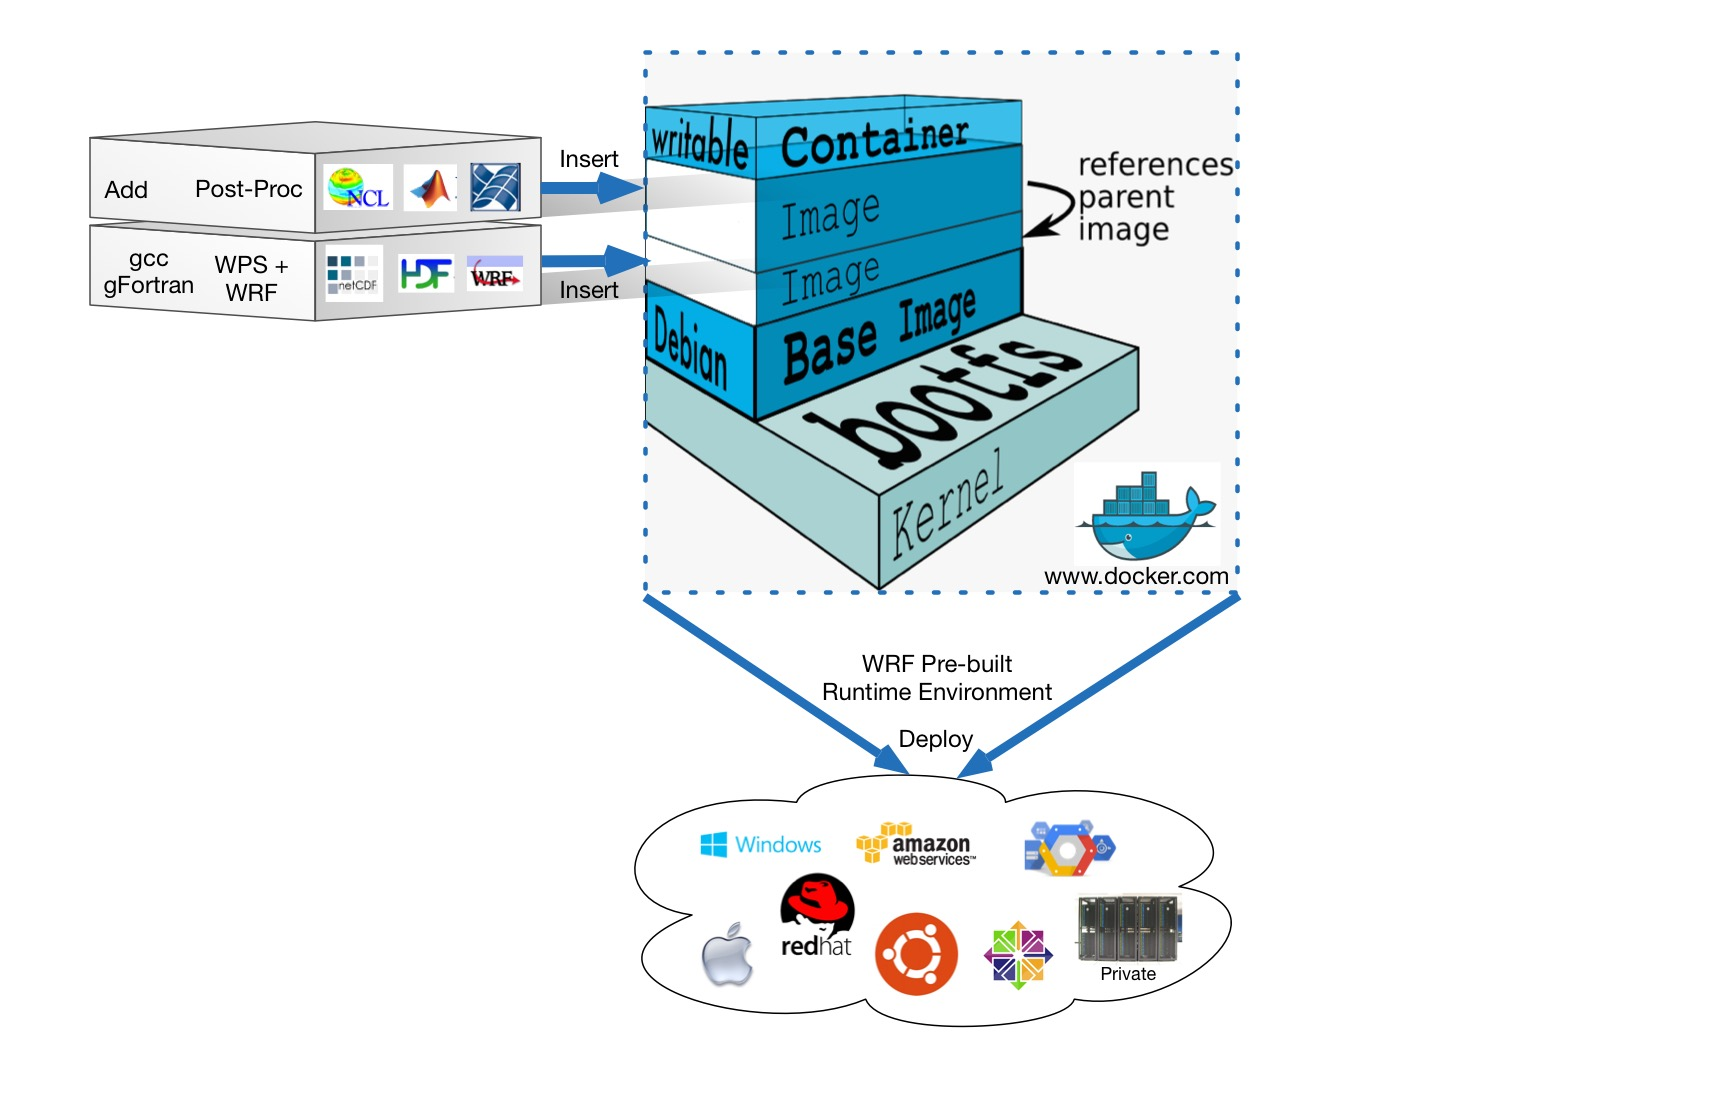
\includegraphics[scale=0.2]{figures/WRF-Docker-Deploy.jpg}
\caption{\label{Fig:Docker} Schematic illustrating the current WRF deployment in a Docker container. It includes initialization (pre-processing via the WRF Preprocessing System WPS) and post-processing graphics with NCAR Command Language (NCL) scripting}
\end{center}
\end{figure}



\section{Uncertainty quantification}

One of the primary reasons that NWP research has been historically non-reproducible is that different computer architectures and environments perform mathematical operations differently.  Differences can be greater in when parallel operations are included.  First, different chips have different binary truncation. Second, compilers sometimes reorder operations in attempts to speed computation; the reordering depends on the compiler brand, version, and level of optimization.  Third, unless carefully implemented parallel computations do not perform operations in the same order.  Often this is not a requirement, but truncation guarantees that some computations are not reproducible when the order of a parallel computation is not enforced. For example, the result of an average depends on the precision in the sum and division, and in which order they are performed.  \citet{Thomas02} provides an example of the effect of compiler optimization and parallel topology on NWP, and \citet{Baker:2015} shows how lack of numerical reproducibility can indicate code quality.

Compiler optimization results.

Need to find an AMD chip, or another, for chip results.

\section{Performance}

Various machines

Docker overhead, VM overhead.

\section{Summary}


%%%%%%%%%%%%%%%%%%%%%%%%%%%%%%%%%%%%%%%%%%%%%%%%%%%%%%%%%%%%%%%%%%%%%
% ACKNOWLEDGMENTS
%%%%%%%%%%%%%%%%%%%%%%%%%%%%%%%%%%%%%%%%%%%%%%%%%%%%%%%%%%%%%%%%%%%%%
%
\acknowledgments
Start acknowledgments here. NSF.

%%%%%%%%%%%%%%%%%%%%%%%%%%%%%%%%%%%%%%%%%%%%%%%%%%%%%%%%%%%%%%%%%%%%%
% APPENDIXES
%%%%%%%%%%%%%%%%%%%%%%%%%%%%%%%%%%%%%%%%%%%%%%%%%%%%%%%%%%%%%%%%%%%%%
%
% Use \appendix if there is only one appendix.
%\appendix

% Use \appendix[A], \appendix}[B], if you have multiple appendixes.
%\appendix[A]

%% Appendix title is necessary! For appendix title:
%\appendixtitle{}

%%% Appendix section numbering (note, skip \section and begin with \subsection)
% \subsection{First primary heading}

% \subsubsection{First secondary heading}

% \paragraph{First tertiary heading}

%% Important!
%\appendcaption{<appendix letter and number>}{<caption>} 
%must be used for figures and tables in appendixes, e.g.,
%
%\begin{figure}
%\noindent\includegraphics[width=19pc,angle=0]{figure01.pdf}\\
%\appendcaption{A1}{Caption here.}
%\end{figure}

%%%%%%%%%%%%%%%%%%%%%%%%%%%%%%%%%%%%%%%%%%%%%%%%%%%%%%%%%%%%%%%%%%%%%
% REFERENCES
%%%%%%%%%%%%%%%%%%%%%%%%%%%%%%%%%%%%%%%%%%%%%%%%%%%%%%%%%%%%%%%%%%%%%
% Make your BibTeX bibliography by using these commands:
 \bibliographystyle{ametsoc2014}
 \bibliography{refs.bib}


%%%%%%%%%%%%%%%%%%%%%%%%%%%%%%%%%%%%%%%%%%%%%%%%%%%%%%%%%%%%%%%%%%%%%
% TABLES
%%%%%%%%%%%%%%%%%%%%%%%%%%%%%%%%%%%%%%%%%%%%%%%%%%%%%%%%%%%%%%%%%%%%%
%% Enter tables at the end of the document, before figures.
%%
%

%%%%%%%%%%%%%%%%%%%%%%%%%%%%%%%%%%%%%%%%%%%%%%%%%%%%%%%%%%%%%%%%%%%%%
% FIGURES
%%%%%%%%%%%%%%%%%%%%%%%%%%%%%%%%%%%%%%%%%%%%%%%%%%%%%%%%%%%%%%%%%%%%%
%% Enter figures at the end of the document, after tables.
%%
%
%\begin{figure}[t]
%  \noindent\includegraphics[width=19pc,angle=0]{figure01.pdf}\\
%  \caption{Enter the caption for your figure here.  Repeat as
%  necessary for each of your figures. Figure from \protect\cite{Knutti2008}.}\label{f1}
%\end{figure}

%\clearpage
%\begin{figure}[t]
%  \noindent\includegraphics[width=19pc,angle=0]{../figs/WRFsolar.eps}\\
% \caption{\label{fig:wrfsolar}Sketch representing the physical processes that WRF-Solar is improving.}
%\end{figure}

\end{document}
